\begin{MyArticle}[enhanced, tikz={rotate=0}, width=0.24\textwidth]{Multi-Muons In CDF: The Mystery Continues}
  \begin{multicols}{2}
    We present a phenomenological conjecture of new physics that is suggested
    by the topology and kinematic properties of the multi-muon events recently
    reported by the CDF collaboration. We show that the salient features of 
    the data can be accounted for by postulating the pair production of
    three new states $h_1$, $h_2$, and $h_3$ with masses in the range
    of 15, 7.3, and 3.6 GeV/c$^{2}$, respectively. The heavier states 
    cascade-decay into the lighter ones, whereas the lightest state 
    decays into a $\tau$ pair with a lifetime of the order of 20 ps.
    \begin{comment}
    % ========================
    \begin{figure}
      \begin{center}
        \vspace{-0.2in}
        \leavevmode
        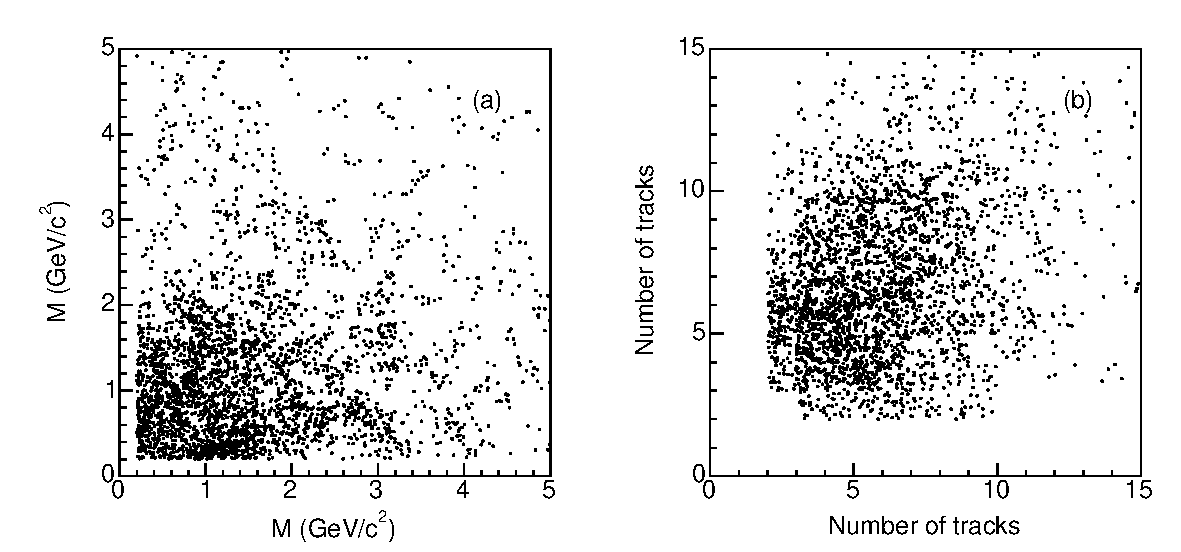
\includegraphics[width=\textwidth]{./figures/MultiMuons2_CDF.pdf}
        %\caption[]{Two-dimensional distributions, reproduced from Ref.~\cite{a0disc},
        %  of (a) the invariant mass, $M$, of all muons and (b) the total
        %  number of tracks contained in a $36.8^{\deg}$ cone when both
        %  cones contain at least two muons.}
      \end{center}
    \end{figure}
    % ========================
    \end{comment}
  \end{multicols}
\end{MyArticle}
